% IEEE conference paper, two column. Compile: see paper/README.md
% Every number comes from docs/evaluation (see the table of sources in paper/README.md).
% Three-seed numbers come from docs/evaluation/three_seed_results.md (script tools/browser_path/three_seed.py); unfinished numbers would be wrapped in \pending{...}.
% Citations are real papers written from memory and each is marked [VERIFY] in refs.bib: check every one before submission.
\documentclass[conference]{IEEEtran}
\usepackage{graphicx}
\usepackage{amsmath,amssymb}
\usepackage{xcolor}
\usepackage{url}
\usepackage{array}

\newcommand{\pending}[1]{{\color{red}\textbf{[#1]}}}
\newcommand{\todo}[1]{{\color{blue}\textbf{[#1]}}}
\newcommand{\signbridge}{\textsc{SignBridge}}

\begin{document}

\title{Offline Accuracy Is Not Webcam Accuracy: Measuring the Deployment Gap in Landmark-Based Indian Sign Language Recognition}

\author{\IEEEauthorblockN{Darshan BG}
\IEEEauthorblockA{Independent researcher\\
Email: \todo{author email}}}

\maketitle

\begin{abstract}
Landmark-based sign language recognizers are usually reported with accuracy on the test split of the dataset they were trained on. We ask what it means once the model runs behind a web browser and a webcam. We train a 1D CNN, a BiGRU and a Transformer on INCLUDE (Indian Sign Language, 262 classes) and run the same test videos through a real browser MediaPipe pipeline in two picture shapes. At the live confidence threshold of 0.7 the CNN answers 0.82 of 100 test videos correctly from stored features and 0.78 from browser landmarks of 16:9 frames, but 0.65 from 4:3 frames and 0.07 when the 4:3 picture aspect is ignored, with 29\,\% confident wrong answers. Most of the loss that remains in 4:3 comes from the black bars of our letterboxed benchmark pictures: filling them with edge pixels lifts 0.59 to 0.73 against 0.77 native on 100 validation videos. A 10\,\% error in the vertical landmark scale costs 10 to 30 points, and signers who appear small in the frame are recognized less reliably. We add a targeted augmentation (vertical scale, landmark noise, hand dropout) and measure its effect on all three architectures over three seeds: for the CNN it removes most of the failure of an unrescaled 4:3 picture (accuracy 0.06 to 0.62), and for all three architectures it shows no clear change offline, in 16:9 or in rescaled 4:3, so the loss in 4:3 remains. We turn the findings into a camera request, a framing guide and a size warning in an open prototype. All numbers are on the authors' predefined split; signer independence is not verified.
\end{abstract}

\begin{IEEEkeywords}
sign language recognition, Indian Sign Language, deployment, distribution shift, MediaPipe, data augmentation
\end{IEEEkeywords}

\section{Introduction}
Sign language recognition from video is a task where reported accuracy is high and deployed accuracy is rarely measured. A common design replaces pixels with body, hand and face landmarks from a pose estimator, which makes models small enough to run in a web page~\cite{lugaresi2019mediapipe,bazarevsky2020blazepose,zhang2020mediapipehands}. The features then look camera independent, and the test split of the training dataset is treated as the answer to how well the system will work. It is not. In a browser the landmarks come from a different camera, picture shape, resolution and distance than in the dataset, and a landmark model is only as invariant to these as its normalization and training make it.

This paper measures that gap for Indian Sign Language (ISL). We use the INCLUDE dataset~\cite{sridhar2020include}, three standard sequence classifiers, and a running prototype, \signbridge{}, that recognizes isolated signs in the browser and signs typed English with a 3D avatar. Our contributions are:
\begin{enumerate}
\item A browser-path benchmark that feeds dataset test videos through the real in-browser MediaPipe Holistic model in two picture shapes and compares it with the offline path and with Python MediaPipe, with paired tests (Sections~\ref{sec:pipeline} and~\ref{sec:gap}).
\item A sensitivity study to vertical landmark scale, noise, hand dropout and signer size, showing that the dominant failure was a picture aspect mismatch that shoulder-width normalization does not remove.
\item A targeted augmentation derived from those measurements on validation data, evaluated on three architectures over three seeds (Section~\ref{sec:aug}).
\item Their conversion into product behavior: a camera request, a framing guide and a size warning (Section~\ref{sec:guidance}), and a full disclosure of every use of the test split (Section~\ref{sec:limits}).
\end{enumerate}

\section{Related Work}
\textbf{Datasets and recognition.} WLASL~\cite{li2020wlasl} and INCLUDE~\cite{sridhar2020include} made isolated sign classification a standard benchmark~\cite{rastgoo2021survey}; skeleton-based methods are among the strongest and cheapest~\cite{jiang2021sam}, and OpenHands collects pose-based models for several languages, including INCLUDE~\cite{selvaraj2022openhands}. ASL Citizen~\cite{desai2023aslcitizen} (\todo{83,399 videos of 2,731 signs by 52 signers, per its abstract; VERIFY}) identifies its signers and so allows signer-disjoint splits, which INCLUDE does not; the 2023 Google Isolated Sign Language Recognition competition~\cite{kaggle2023islr} made landmark-based recognition an open benchmark \todo{VERIFY the description of the task and data}. These works evaluate held-out splits of the same collection; we evaluate the path a user would run, with MediaPipe~\cite{lugaresi2019mediapipe,bazarevsky2020blazepose,zhang2020mediapipehands} used unchanged on both sides.

\textbf{Shift, augmentation and abstention.} Train-test mismatch is long studied~\cite{quinonero2009dataset,torralba2011bias,koh2021wilds,hendrycks2019robustness,damour2022underspecification}; our shifts are physical (picture aspect, subject size, detector dropout), so we can measure them one at a time and choose an augmentation from the measurements~\cite{shorten2019augmentation}. A reject option trades coverage for accuracy~\cite{geifman2017selective} and needs meaningful confidence~\cite{guo2017calibration}. Technology that claims to translate sign language must be evaluated with signers and their communities~\cite{bragg2019interdisciplinary}; Section~\ref{sec:limits} states what we could not do.

\section{Dataset and Models}\label{sec:data}
\textbf{Data.} INCLUDE contains 4,284 processed videos of 262 classes in the version we use (4 to 25 videos per class, median 15), with the authors' predefined split of 3,121 training, 347 validation and 816 test samples~\cite{sridhar2020include}. INCLUDE lists 263 classes; we use 262. The eight listed videos of one class (``Second (Number)'') are not in the released archives, so that class has no sample. No video appears in two splits. The dataset carries no signer identifiers, so \emph{every result in this paper is on the authors' predefined split and signer independence is not verified.}

\textbf{Features.} Each frame has 225 values: 33 pose, 21 left-hand and 21 right-hand landmarks with $(x,y,z)$. Coordinates are translated so that the shoulder midpoint is the origin and divided by the two-dimensional shoulder distance computed from the normalized image coordinates. A missing hand is an all-zero block; in the stored features 19.6\,\% of frames lack the left hand and 29.6\,\% the right hand. Face landmarks are not used. Sequences are resampled to 32 frames after interpolating hand gaps of at most three frames; the same function serves training and inference.

\textbf{Models.} We train a 1D CNN (343,558 parameters), a bidirectional GRU~\cite{cho2014gru,schuster1997birnn} (636,422) and a Transformer encoder~\cite{vaswani2017attention} (360,710) with identical settings: at most 60 epochs, patience 10 on validation macro-F1, batch size 16, learning rate $10^{-3}$, hidden size 128, two layers, dropout 0.3, seed 0. During training every batch also receives Gaussian noise of standard deviation 0.01 on all 225 input values; the values are in normalized units (shoulder widths), so this is about 0.0013 of the picture width at the median INCLUDE shoulder width of 0.133, and it is added to every value, including $z$ and the all-zero blocks of missing hands. Model selection used the validation split only; each model was evaluated on the test split once.

\begin{table}[t]
\caption{Baseline models on the INCLUDE test split (816 samples), authors' predefined split, signer independence not verified. Accuracy at confidence threshold 0.7 is the answered share and the accuracy among answered.}
\label{tab:base}
\centering
\small
\setlength{\tabcolsep}{4pt}
\begin{tabular}{lcccc}
\hline
Model & Top-1 & Top-5 & Macro-F1 & Cov. / acc. at 0.7\\
\hline
1D CNN & 0.9130 & 0.9902 & 0.9107 & 0.8676 / 0.9548\\
BiGRU & 0.7929 & 0.9730 & 0.7869 & 0.7279 / 0.9074\\
Transformer & 0.7328 & 0.9596 & 0.7100 & 0.7549 / 0.8279\\
\hline
\end{tabular}
\end{table}

Table~\ref{tab:base} gives the standard offline numbers. For orientation, the pose-based baseline listed for INCLUDE in the OpenHands study~\cite{selvaraj2022openhands} is an XGBoost model on OpenPose keypoints~\cite{sridhar2020include} with a top-1 accuracy of \todo{63.10 percent, VERIFY}, and OpenHands reports \todo{91.2 percent for ST-GCN and 93.5 percent for SL-GCN, VERIFY} on INCLUDE (read from the arXiv version). Our CNN (0.9130) is far above the former and within the range of the graph models. The comparison is loose: 262 of 263 classes, MediaPipe instead of OpenPose or HRNet keypoints, our own settings, one seed, and the authors' split in all cases without signer independence. A prediction whose top confidence is below a threshold is reported as UNRECOGNIZED. The live threshold is the lowest value of $\{0, 0.3, 0.5, 0.7, 0.8, 0.9, 0.95\}$ that gives at least 95\,\% accuracy on answered \emph{validation} samples of the best model; for the CNN this is 0.7 (validation coverage 0.8818, accuracy on answered 0.9608). Because the CNN is the model deployed, most single-model experiments below use it, and Section~\ref{sec:aug} extends them to all three.

\section{Browser Deployment Pipeline}\label{sec:pipeline}
The prototype runs MediaPipe Holistic in the browser (WebAssembly, CPU inference, model complexity 0) on frames from the webcam. Only landmarks leave the page: a short buffer (the newest 60 frames, dropped after 15 frames without a body pose) is sent over a WebSocket to a FastAPI server that applies exactly the normalization and resampling of training and returns a label or UNRECOGNIZED. No video is stored or transmitted. Fig.~\ref{fig:pipeline} summarizes the path.

\begin{figure}[t]
\centering
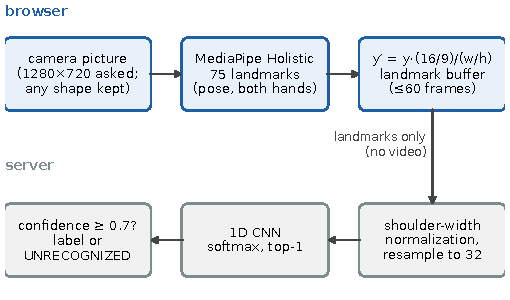
\includegraphics[width=\columnwidth]{figures/fig_pipeline.pdf}
\caption{Browser deployment pipeline. Only landmarks leave the page; $w/h$ is the camera picture's aspect (Eq.~(1)).}
\label{fig:pipeline}
\end{figure}

\textbf{A picture aspect problem.} MediaPipe returns $x$ as a fraction of the picture width and $y$ as a fraction of its height. INCLUDE videos are 16:9; a webcam is commonly 4:3. A vertical distance of $d$ pixels next to a shoulder width of $s$ pixels appears in the landmarks as $(d/H)/(s/W)=(d/s)\,(W/H)$, where $W/H$ is the picture aspect. In a 4:3 picture the normalized vertical distances of the same pose are therefore smaller than in a 16:9 picture by $(4/3)/(16/9)=0.75$, and the shoulder-width normalization (which uses the 2D distance) does not undo this because it divides $x$ and $y$ by the same number. An unrescaled 4:3 camera thus behaves like a 16:9 camera whose vertical coordinates are multiplied by 0.75. We multiply the vertical coordinate of every landmark by the inverse, $4/3$ for a 4:3 camera, which gives what the same pose would give in a 16:9 picture,
\begin{equation}
y' = y\cdot\frac{16/9}{w/h},
\end{equation}
with $w/h$ the camera picture's aspect, before it is sent (Section~\ref{sec:guidance} describes the camera request). $x$ and $z$ are unchanged. The rescale is exact in the sense that, in normalized coordinates, it equals the effect of scaling the raw $y$ by $s$ and re-normalizing, which we use to implement the augmentation of Section~\ref{sec:aug} on stored features.

\section{Deployment-Gap Experiments}\label{sec:gap}
\textbf{Protocol.} We took test videos of the authors' predefined split whose original file is available, one per class, drawn with a fixed seed: 100 videos for the CNN study reported in this section, and a separate validation set of 100 videos for tuning decisions. Each video was resized to 1280$\times$720 (16:9) and, separately, letterboxed into 640$\times$480 (4:3); every third frame (8 to 10 frames per second) was written as a JPEG, and a headless Chrome instance passed the frames one at a time to the prototype's self-hosted MediaPipe Holistic (smoothing on, CPU inference). We compare: (a) \emph{offline}, the stored features of the same videos; (b) \emph{Python} MediaPipe on the same JPEG frames; (c) \emph{browser} landmarks, with and without the vertical rescale. Accuracy is the share of videos answered above the threshold \emph{and} correct; wrong-accepted is answered above the threshold and wrong; the remainder is UNRECOGNIZED. Intervals are 95\,\% Wilson intervals~\cite{wilson1927}; paired comparisons use the exact McNemar test (an exact binomial test on the discordant videos)~\cite{mcnemar1947}. The body pose was found in every frame in all sources and hands in about 87\,\%, so detection loss is not what is measured. The harness has no user-interface code, camera or socket, and one sample per class gives intervals of about $\pm 9$ points.


\subsection{Browser against offline}
Table~\ref{tab:bvo} shows the main result. In native 16:9 the browser path is within noise of the offline path: 0.78 against 0.82 (6 videos lost and 2 gained, $p=0.29$), with a wrong-accepted rate of 0.02. In 4:3 the loss is large: 0.65 (22 videos lost, 5 gained, $p=0.002$), with 0.07 wrong accepted and 0.28 UNRECOGNIZED. Python MediaPipe on the same 4:3 frames reaches 0.70, so most of the loss comes from the input, not the browser build; on identical frames the browser is 3 to 5 points below Python, which is not significant at this sample size.

\begin{table}[t]
\caption{CNN, 100 test videos, threshold 0.7 (authors' predefined split, signer independence not verified). Acc.\ = correct and accepted with 95\,\% Wilson interval; WA = wrong accepted; UN = unrecognized; Top-1 ignores the threshold.}
\label{tab:bvo}
\centering
\small
\begin{tabular}{lccccc}
\hline
Source & Acc. & (interval) & WA & UN & Top-1\\
\hline
Offline features & 0.82 & 0.73 to 0.88 & 0.03 & 0.15 & 0.92\\
Python, 16:9 & 0.81 & 0.72 to 0.87 & 0.03 & 0.16 & 0.90\\
Browser, 16:9 & 0.78 & 0.69 to 0.85 & 0.02 & 0.20 & 0.87\\
Python, 4:3 & 0.70 & 0.60 to 0.78 & 0.05 & 0.25 & 0.81\\
Browser, 4:3 & 0.65 & 0.55 to 0.74 & 0.07 & 0.28 & 0.78\\
Python, 4:3 raw & 0.08 & & 0.29 & 0.63 & 0.12\\
Browser, 4:3 raw & 0.07 & & 0.29 & 0.64 & 0.10\\
\hline
\end{tabular}
\end{table}

Without the vertical rescale, 4:3 input gives 0.07 accuracy and 29\,\% confident wrong answers: the model fails not by hesitating but by answering wrongly. Two diagnostics separate resolution from shape. A 16:9 picture resized to 640$\times$360 gives 0.80, so a smaller picture is not the cause. A centre crop of the 16:9 frame to 4:3 (a webcam-like fill) with the rescale gives 0.76, six points below 16:9, so a real webcam probably lies between the letterboxed and the native result; we did not measure a real webcam with real signers.

The loss that remains in 4:3 after the exact rescale (0.65 against 0.78 in 16:9 on the test videos, 0.58 against 0.75 on the validation videos) is \emph{not explained} by any factor we measured. It is not a vertical scale error: the rescale is exact, and the sweep of Fig.~\ref{fig:y} shows how large a mismatch would have to be to matter. It is not signer size: letterboxing keeps the picture width, so the shoulder width as a fraction of the width is unchanged. It is not resolution: a 640$\times$360 16:9 picture scores 0.80. The remaining candidate is the black padding of the letterbox, which we test next.

\textbf{Does black padding explain the residual loss?} We classified the sampled frames of the 100 validation videos with Python MediaPipe in six picture variants (Table~\ref{tab:pad}); the vertical rescale is applied to every picture that is not 16:9. A hand was found in 84 to 85\,\% of the frames in every variant, so the detection rate does not differ. The black letterbox scores 0.59, 18 points below the native picture (19 videos lost and 1 gained, exact McNemar $p<0.001$) and 13 points below a 16:9 picture of the same 640$\times$360 resolution (0.72, $p=0.011$). Filling the bars with replicated edge pixels instead of black raises the score to 0.73 (19 videos gained and 5 lost against the black letterbox, $p=0.007$), which is indistinguishable from the same-resolution 16:9 picture (3 and 4 videos, $p=1.0$) and 4 points below native ($p=0.22$). A taller black frame (1:1) does not lose more (0.61 against 0.59, $p=0.69$). In this benchmark, black padding therefore explains most of the residual 4:3 loss and picture resolution a smaller part. An unpadded 4:3 centre crop reaches 0.68, below native ($p=0.012$), but it enlarges the signer by 4/3 (shoulder width about 0.18, above the 0.15 covered by the signer-size study below) and cuts the sides of the picture, so it cannot separate those factors from padding. Caveats: these are Python landmarks (the browser's letterboxed accuracy on the same videos, 0.58, is close to Python's 0.59), and a real 4:3 webcam picture has no bars, so the letterboxed benchmark probably overstates the 4:3 loss on real cameras, which we did not measure.

\begin{table}[t]
\caption{Padding test: 100 validation videos, Python MediaPipe, baseline CNN, threshold 0.7 (authors' predefined split, signer independence not verified). Acc.\ = correct and accepted with a 95\,\% Wilson interval; WA = wrong accepted.}
\label{tab:pad}
\centering
\small
\setlength{\tabcolsep}{2.5pt}
\begin{tabular}{lccc}
\hline
Picture & Acc. & WA & Top-1\\
\hline
Native 16:9 & 0.77 (0.68 to 0.84) & 0.02 & 0.86\\
16:9, 640$\times$360 & 0.72 (0.63 to 0.80) & 0.04 & 0.86\\
4:3 letterbox, black & 0.59 (0.49 to 0.68) & 0.06 & 0.71\\
4:3 letterbox, edge fill & 0.73 (0.64 to 0.81) & 0.05 & 0.82\\
1:1 letterbox, black & 0.61 (0.51 to 0.70) & 0.07 & 0.73\\
4:3 centre crop & 0.68 (0.58 to 0.76) & 0.06 & 0.83\\
\hline
\end{tabular}
\end{table}

\textbf{Per-sign loss.} On the 211 validation videos (165 signs) and the three baseline CNN seeds, 100 of the 633 video-seed pairs went from correct in 16:9 to not correct in the rescaled letterboxed 4:3 picture, and 23 went the other way. Fish (6 of 6 lost), Election, Sign and Sport (3 of 3 each), Bus, Colour, Dog, Grey and Pink (3 of 5 or 6 each) lose most. Vertical hand movement range (95th minus 5th percentile of wrist height, in shoulder widths) does not explain it: the Spearman correlation with the loss is $-0.10$ (permutation $p=0.16$, 211 videos), and the median range is 3.0 for videos lost in at least one seed and 3.3 for the others. With one or two videos per sign this is descriptive, and it was measured on the padded pictures.

\subsection{Vertical scale, noise and hand dropout}
We applied controlled perturbations to the browser landmarks of 100 \emph{validation} videos (Fig.~\ref{fig:y}). With no perturbation the CNN scores 0.75 in 16:9 and 0.58 in 4:3. A vertical scale error of 10\,\% lowers the 16:9 accuracy to 0.43 (factor 0.9) or 0.65 (1.1); 25\,\% leaves 0.26 with 36\,\% wrong accepted, and a factor 0.75, which is exactly what an unrescaled 4:3 camera produces, leaves 0.05. The model is therefore very sensitive to a cue that shoulder-width normalization cannot remove. Noise and dropout cost accuracy gradually, whereas vertical scale is a cliff: noise of 0.002, 0.005, 0.01 and 0.02 of the picture size gives accuracy 0.74, 0.72, 0.70 and 0.44 (wrong accepted 0.02 to 0.11), and removing each hand in 10, 20, 40 and 60\,\% of the frames gives 0.77, 0.69, 0.55 and 0.30 (wrong accepted 0.02 to 0.16). The browser already misses a hand in about 13\,\% of frames, so the dropout rates of 10 to 20\,\% are within what a live camera produces.


\begin{figure}[t]
\centering
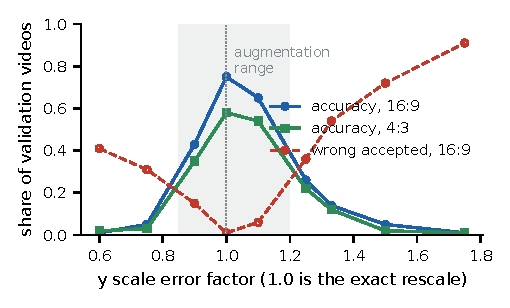
\includegraphics[width=\columnwidth]{figures/fig_yscale.pdf}
\caption{CNN accuracy and wrong-accepted rate against a vertical scale error applied to browser landmarks of 100 validation videos (authors' predefined split, signer independence not verified). The shaded band is the range used for augmentation in Section~\ref{sec:aug}.}
\label{fig:y}
\end{figure}

\subsection{Signer size in the picture}
To test framing, we shrank 30 validation videos toward the picture centre (to 100, 60, 45 and 30\,\% of their size, black padding, aspect unchanged) and classified Python landmarks of the result, binned by the median shoulder width as a fraction of the picture width (Fig.~\ref{fig:frame}). INCLUDE signers measure 0.116 to 0.149 (median 0.133). Accuracy is 0.89 for widths of 0.13 to 0.17 and 0.83 for 0.10 to 0.13, falls to 0.71 for 0.08 to 0.10 and to 0.59 and 0.50 below 0.08, where 12 to 14\,\% of answers are confidently wrong. At 30\,\% size no body pose was found. No width above 0.15 is covered, so a signer who fills the frame is unmeasured. The bins are rough (12 to 32 video-size pairs each). Cropping toward the signer (shoulder widths 0.175 to 0.259) lowered accuracy to 0.30 to 0.43, but the crop also cut the hands off (a hand in only 33 to 63\,\% of frames against about 87\,\%), so size and lost hands cannot be separated and sizes above 0.15 stay untested.

\begin{figure}[t]
\centering
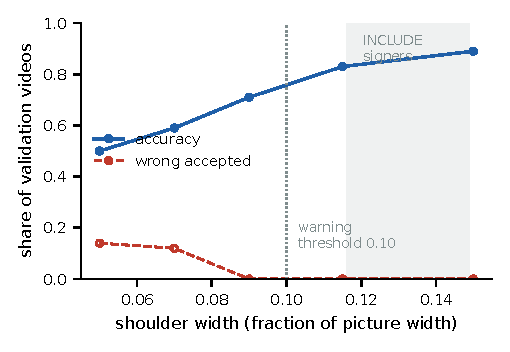
\includegraphics[width=\columnwidth]{figures/fig_framing.pdf}
\caption{CNN accuracy and wrong-accepted rate against median shoulder width (fraction of picture width), validation videos shrunk toward the centre, Python MediaPipe (authors' predefined split, signer independence not verified). The dotted line is the warning threshold of the prototype.}
\label{fig:frame}
\end{figure}

\subsection{Other architectures}
Table~\ref{tab:arch} repeats the browser-path conditions for the BiGRU and the Transformer, with three seeds each, on the larger test corpus (312 videos, one or two per class). The CNN is the best architecture in every condition; the Transformer's validation-chosen threshold is 0.95, so it answers few videos at that threshold. Every baseline loses accuracy in rescaled 4:3 (by 0.13, 0.10 and 0.05 on average) and the unrescaled picture is again a collapse for the CNN ($0.06\pm0.02$).

\begin{table*}[t]
\caption{Three seeds on the 312 test videos of the browser corpus (authors' predefined split, signer independence not verified). Baseline: mean $\pm$ SD of the accuracy at each model's validation-chosen threshold over seeds 0, 1 and 2. Change: augmented minus baseline of the same seed, mean and 95\,\% $t$-interval over the three differences; bold if the interval excludes zero, otherwise there is no clear change. The gap row gives the mean baseline gap and the change of the gap. Each trained model is evaluated once on these videos.}
\label{tab:arch}
\centering
\footnotesize
\setlength{\tabcolsep}{3pt}
\begin{tabular}{lcccccc}
\hline
 & \multicolumn{2}{c}{1D CNN} & \multicolumn{2}{c}{BiGRU} & \multicolumn{2}{c}{Transformer}\\
Condition & Baseline & Change & Baseline & Change & Baseline & Change\\
\hline
Offline features & 0.85 $\pm$ 0.03 & $-0.05$ ($-0.26$ to $+0.16$) & 0.62 $\pm$ 0.10 & $+0.09$ ($-0.36$ to $+0.54$) & 0.38 $\pm$ 0.08 & $-0.08$ ($-0.51$ to $+0.36$)\\
Browser, 16:9 & 0.84 $\pm$ 0.05 & $-0.06$ ($-0.25$ to $+0.13$) & 0.57 $\pm$ 0.11 & $+0.07$ ($-0.44$ to $+0.58$) & 0.36 $\pm$ 0.07 & $-0.07$ ($-0.49$ to $+0.35$)\\
Browser, 4:3 with rescale & 0.71 $\pm$ 0.05 & $-0.04$ ($-0.23$ to $+0.15$) & 0.47 $\pm$ 0.08 & $+0.07$ ($-0.35$ to $+0.49$) & 0.31 $\pm$ 0.06 & $-0.05$ ($-0.43$ to $+0.33$)\\
Browser, 4:3 raw & 0.06 $\pm$ 0.02 & \textbf{$+0.57$ ($+0.26$ to $+0.88$)} & 0.38 $\pm$ 0.07 & $+0.13$ ($-0.19$ to $+0.44$) & 0.20 $\pm$ 0.05 & $+0.03$ ($-0.30$ to $+0.36$)\\
Wrong accepted, browser 16:9 & 0.04 $\pm$ 0.00 & $0.00$ ($-0.06$ to $+0.07$) & 0.02 $\pm$ 0.01 & $+0.02$ ($-0.04$ to $+0.08$) & 0.04 $\pm$ 0.02 & $-0.02$ ($-0.04$ to $0.00$)\\
Gap 16:9 minus 4:3 (rescaled), change & 0.13 & $-0.02$ ($-0.12$ to $+0.09$) & 0.10 & $0.00$ ($-0.09$ to $+0.09$) & 0.05 & $-0.02$ ($-0.06$ to $+0.02$)\\
Chosen threshold, seeds 0, 1, 2 & 0.7, 0.7, 0.7 & aug.: 0.9, 0.5, 0.7 & 0.9, 0.9, 0.9 & aug.: 0.7, 0.9, 0.9 & 0.95, 0.95, 0.95 & aug.: 0.95, 0.95, 0.95\\
\hline
\end{tabular}
\end{table*}

\section{Targeted Augmentation}\label{sec:aug}
\textbf{Design.} The measurements of Section~\ref{sec:gap} on validation videos fix three augmentations, all applied to the stored normalized features of each training sample at every epoch. (i) \emph{Vertical scale}: with probability 0.8 the raw $y$ is multiplied by a factor drawn uniformly from 0.85 to 1.20 and the coordinates are re-normalized with the new shoulder distance; this is exact and is tested against re-normalizing scaled raw landmarks. The range is a margin of about 10\,\% around the exact rescale. (ii) \emph{Landmark noise}: independent Gaussian jitter on $x$ and $y$ of every detected landmark, with a per-sample standard deviation drawn from 0 to 0.01 of the picture size (converted to normalized units with the median INCLUDE shoulder width, 0.133); missing hands stay exactly zero. This differs from the baseline input noise of Section~\ref{sec:data} in three ways: it is up to about 7.5 times larger (0.01 of the picture size is about 0.075 normalized units, against 0.01), its size is drawn per sample instead of being fixed, and it never touches $z$ or the zero blocks of missing hands, so the presence of a hand stays an unambiguous signal. The baseline noise is kept in all runs, so the augmented models receive both. (iii) \emph{Hand dropout}: each hand in each frame is zeroed with a per-sample probability drawn from 0 to 0.2. Nothing else changes: same split, seed handling, settings and checkpoint rule as the baseline.

\textbf{Evaluation.} Each of the three architectures is trained with and without the augmentation, for three seeds. We report the offline and browser-path conditions of Table~\ref{tab:arch} and the difference between each augmented model and the baseline of the same seed, with a 95\,\% $t$-interval over the three differences (an interval that contains zero is read as no clear change). The perturbation sweeps were run for seed 0 only.


\textbf{Results.} The augmentation clearly helps in one case, the one it was designed for: for the CNN it lifts the accuracy of the unrescaled 4:3 picture from 0.06 to 0.62 (change $+0.57$, interval $+0.26$ to $+0.88$). In every other cell of Table~\ref{tab:arch}, offline, 16:9 and rescaled 4:3 for all three architectures and the unrescaled picture for the BiGRU and the Transformer, the interval contains zero: there is no clear change, and also no clear regression, although the spread between seeds is large (the BiGRU's differences in 16:9 are $+0.30$, $-0.09$ and $0.00$). The BiGRU's top-1 accuracy on the unrescaled picture rises by $+0.12$ ($+0.01$ to $+0.23$). The gap between 16:9 and rescaled 4:3 does not change clearly for any architecture, as expected from a padding effect that the augmentation does not address (Section~\ref{sec:gap}-A). The unrescaled picture with an augmented CNN (0.62) still scores below the rescaled picture with the baseline (0.71), so the augmentation does not replace the rescale. The perturbation sweeps (seed 0, validation videos only) give no conclusion either: the augmentation raised the CNN's accuracy at vertical scale errors of 0.9 and 1.25 but lowered it with noise and hand dropout, and they were not repeated for other seeds.

\textbf{Threshold trade-off.} Augmentation changes how confident a model is, so the validation-chosen threshold may change. Table~\ref{tab:trade} shows, for seed 0, the coverage and accuracy trade-off of the baseline CNN offline (816 test samples), in the browser path (312 test videos, 16:9) and of the augmented CNN offline. At 0.7 the browser path answers 0.82 of the videos against 0.87 offline, with the same accuracy on the answered ones (0.95), so the browser abstains more rather than answering worse. The augmented CNN answers slightly more (0.88) at a similar accuracy (0.95), but its validation-chosen thresholds differ between seeds (0.9, 0.5 and 0.7), so a threshold is a per-model choice.

\begin{table}[t]
\caption{Coverage and accuracy on answered samples against the confidence threshold, seed 0 (authors' predefined split, signer independence not verified): baseline CNN offline on the 816 test samples, the same model in the browser path on 312 test videos in 16:9, and the augmented CNN offline.}
\label{tab:trade}
\centering
\small
\setlength{\tabcolsep}{3pt}
\begin{tabular}{lccc}
\hline
Threshold & Offline CNN & Browser 16:9 & Augmented CNN\\
 & cov. / acc. & cov. / acc. & cov. / acc.\\
\hline
0.50 & 0.9559 / 0.9346 & 0.9359 / 0.9075 & 0.9559 / 0.9256\\
0.70 & 0.8676 / 0.9548 & 0.8205 / 0.9531 & 0.8775 / 0.9483\\
0.80 & 0.8162 / 0.9700 & 0.7788 / 0.9588 & 0.8248 / 0.9614\\
0.90 & 0.7451 / 0.9770 & 0.7051 / 0.9682 & 0.7304 / 0.9681\\
0.95 & 0.6556 / 0.9757 & 0.6090 / 0.9684 & 0.6299 / 0.9786\\
\hline
\end{tabular}
\end{table}

\textbf{Calibration.} A threshold needs meaningful confidence. On the 211 validation videos (10 bins, baseline CNN) the expected calibration error is 0.04 offline (0.03 to 0.06 over three seeds), 0.04 in browser 16:9 (0.03 to 0.04) and 0.07 in rescaled 4:3 (0.04 to 0.07). Without the rescale it is 0.52 to 0.65: the mean confidence stays at 0.61 to 0.73 while top-1 accuracy is 0.07 to 0.09, so a threshold cannot catch that failure. These are rough estimates on the split that chose the threshold.

\section{Framing Guidance}\label{sec:guidance}
Three measurements became product behavior. The prototype requests 1280$\times$720 from the camera, adapts to the camera's actual shape and, for any non-16:9 camera, applies the rescale of Section~\ref{sec:pipeline}. It draws a dashed outline for head, shoulders and hands with the shoulders at about 14\,\% of the width, inside the tested range (INCLUDE signers measure 0.12 to 0.15). And it warns when the smoothed shoulder width falls below 0.10 of the picture width: in Fig.~\ref{fig:frame} accuracy is 0.83 or more at 0.10 and above, 0.71 between 0.08 and 0.10 and about 0.55 below. These choices rest on validation videos, not on real users, and the guide does not ask the signer to move closer than the tested range.

\section{Case Study: SignBridge}\label{sec:case}
\signbridge{} is an open prototype with five tabs: conversation, sign to English (isolated and continuous), English to sign, a recorder for the signer's own takes, and a landmark check of browser against Python landmarks. The frontend is Next.js with a React Three Fiber avatar and the backend FastAPI with PyTorch. English to sign uses a rule-based gloss converter and avatar clips retargeted automatically from INCLUDE landmark samples; \emph{no clip is reviewed by a signer}. Continuous mode splits 98.1\,\% of signs correctly on streams joined from real INCLUDE samples with 10 rest frames between signs, and only 75.2\,\% with natural margins alone. The prototype follows the findings above: landmarks only, rescale by picture aspect, a 16:9 camera request, a small-framing warning, and UNRECOGNIZED below the validated threshold.

\section{Limitations}\label{sec:limits}
\textbf{Split and signers.} All results use the authors' predefined split without signer identifiers, so a person may appear in training and test; absolute accuracies are optimistic for new signers and the gap we measure is a lower bound for unseen people.

\textbf{No face features.} Face landmarks are not used, although facial expression carries grammar in ISL (questions, negation); the avatar's head movements for these are rule-based approximations.

\textbf{Residual 4:3 gap.} Vertical scale, signer size and resolution do not explain the loss that remains in 4:3 after the rescale; black padding does most of it on validation videos (Section~\ref{sec:gap}), but that used Python landmarks and one fill, the unpadded crop is confounded by signer size, and a real 4:3 webcam has no bars, so the loss on real cameras is unmeasured.

\textbf{Real webcams.} All browser results use dataset videos re-encoded as pictures: no real webcam, lighting, users or left-handed signer, and the framing study covers sizes up to the dataset range only. One or two videos per class give wide intervals, and the 100-video CNN study of Section~\ref{sec:gap} is a single seed (the three-seed table is on a larger corpus).

\textbf{Licence.} INCLUDE is CC BY 4.0 in the Zenodo record and CC BY-NC-SA 4.0 on a third-party page; we follow the stricter reading for everything derived from it (non-commercial, attribution, share alike), and data, weights and clips are not in the public repository. The avatar character's licence terms are unconfirmed and it is not distributed.

\textbf{Test-split disclosure.} The test split was used as follows; we list every use known to us.
\begin{enumerate}
\item The three baseline models (seed 0) were each evaluated once on the full test split (816 samples) for Table~\ref{tab:base}; the earlier pilot runs never read test features.
\item The segmentation study of Section~\ref{sec:case} evaluated streams of test samples once per rest-gap setting (three settings) after tuning on validation.
\item The browser-path benchmark of the baseline CNN on 100 test videos (Section~\ref{sec:gap}) followed three fake-camera runs on three INCLUDE test videos whose wrong results first exposed the picture-aspect problem; the rescale was therefore designed after seeing test videos, although it was derived from the geometry and its size was not tuned on test data.
\item After a speed-up of the resampling routine, the baseline CNN was run over the test split once to confirm that its accuracy (0.9130) was unchanged.
\item Each of the three augmented models (seed 0) and each of the twelve additional models (seeds 1 and 2, baseline and augmented) was evaluated once on the full test split at the end of its training run.
\item The 312 test videos of the larger browser corpus were used once per trained model in Table~\ref{tab:arch}: the six seed-0 models and the twelve further models (eighteen evaluations).
\end{enumerate}
No augmentation range, threshold or model choice was tuned on the test split; they were chosen on validation data (Section~\ref{sec:gap} and the validation sweeps).

\section{Conclusion}
A landmark recognizer that answers 0.82 of 100 test videos correctly from stored features (0.92 top-1) answers only 0.07 of the same videos correctly (0.10 top-1), with 29\,\% confident wrong answers, when it receives landmarks from a 4:3 picture whose aspect is ignored. A geometric rescale removes that failure. The loss that remains in 4:3 (0.65 against 0.82 offline for the CNN) was traced mostly to the black bars of our letterboxed pictures in a validation test, so the loss on real 4:3 cameras is unmeasured; accuracy is also very sensitive to vertical scale and lower for signers who appear small. A targeted augmentation, evaluated over three seeds, removes most of the unrescaled-4:3 failure for the CNN but shows no clear change elsewhere and does not replace the rescale. The central lesson is methodological: report the accuracy of the path a user will run, with picture shape, framing and abstention rule stated, on a split whose signer independence is known. The next step is recording signers under their own identifiers on real webcams and reviewing the avatar clips with Deaf signers.

\section*{Ethics Statement}
This work uses only the public INCLUDE videos and split lists, under the licence terms above; no new video of any person was collected and none is redistributed. The prototype sends landmarks only and stores no video. The study has no Deaf co-author or reviewer and no signer reviewed the avatar clips. The prototype is not an interpreting service and must not be used where an error could harm a person; no claim here concerns unseen signers.

\section*{Code Availability}
Code, scripts and per-video results: \url{https://github.com/DarshanCat/-SignBridge} (MIT licence; \todo{confirm the repository is public and up to date}). INCLUDE data, features, weights and avatar assets are not included; see the repository's data notice.

\section*{Acknowledgment}
We thank the INCLUDE authors for the dataset. \todo{add acknowledgments}

\bibliographystyle{IEEEtran}
\bibliography{refs}

\end{document}
